% =============================================================================
% IOPS -- one-slide advertisement (~2 minute lightning pitch)
% Self-contained: compile with  pdflatex iops_advert.tex
% =============================================================================
\documentclass[aspectratio=169,11pt]{beamer}

\usetheme{metropolis}

% ---- Fonts (Fira, pdflatex-friendly) ---------------------------------------
\usepackage[T1]{fontenc}
\usepackage[utf8]{inputenc}
\usepackage[sfdefault,scaled=.95]{FiraSans}
\usepackage{FiraMono}
\usepackage{newtxsf}

\usepackage{tcolorbox}
\usepackage{fontawesome5}
\usepackage{tikz}

% ---- Palette (matches the main IOPS deck) ----------------------------------
\definecolor{iopsNavy}{HTML}{16323F}
\definecolor{iopsBlue}{HTML}{1F8FD0}
\definecolor{iopsCyan}{HTML}{49B4E6}
\definecolor{iopsSky}{HTML}{EAF5FC}
\definecolor{iopsPink}{HTML}{E0356E}
\definecolor{iopsGrey}{HTML}{6A7A86}

\setbeamercolor{normal text}{fg=iopsNavy, bg=white}
\setbeamercolor{background canvas}{bg=white}
\setbeamercolor{frametitle}{bg=white, fg=iopsNavy}
\setbeamercolor{progress bar}{fg=iopsBlue, bg=iopsSky}
\setbeamercolor{title separator}{fg=iopsBlue}
\metroset{progressbar=none, numbering=none}
\setbeamertemplate{footline}{}
\setbeamersize{text margin left=6mm, text margin right=6mm}

% ---- Reusable bits ---------------------------------------------------------
\newcommand{\hl}[1]{{\color{iopsPink}\bfseries #1}}
\newtcolorbox{keybox}[1][]{colback=iopsSky, colframe=iopsBlue,
  boxrule=0.6pt, arc=2pt, left=5pt, right=5pt, top=3pt, bottom=3pt, #1}
\newtcbox{\chip}{on line, colback=iopsSky, colframe=iopsBlue, boxrule=0.5pt,
  arc=3pt, left=3pt, right=3pt, top=1pt, bottom=1pt, fontupper=\footnotesize,
  nobeforeafter}

\begin{document}

\begin{frame}[plain]
  \vspace*{2mm}
  % --- Title block with logo on the right -----------------------------------
  \begin{columns}[c]
    \begin{column}{0.82\textwidth}
      {\LARGE\bfseries\color{iopsNavy} IOPS}\quad
      {\normalsize\color{iopsBlue} Reproducible benchmarking, from one YAML to a report}\\[1pt]
      {\footnotesize\color{iopsGrey} Integrated Orchestration for Parametric Studies}
    \end{column}
    \begin{column}{0.18\textwidth}
      \hfill
\includegraphics[height=1.15cm]{logo.png}
    \end{column}
  \end{columns}
  \vspace{1pt}
  {\color{iopsBlue}\rule{\textwidth}{1pt}}
  \vspace{4pt}

  \begin{columns}[c]
    % --- Left: the pitch ----------------------------------------------------
    \begin{column}{0.42\textwidth}
      {\scriptsize\bfseries Describe the study once in YAML. IOPS does the rest:}
      \begin{itemize}\setlength\itemsep{4pt}
        \item[\textcolor{iopsBlue}{\faRandom}] {\scriptsize Sweep: exhaustive, random, \hl{Bayesian}, adaptive}
        \item[\textcolor{iopsBlue}{\faServer}] {\scriptsize Run \hl{locally or on SLURM}, cached, repeated}
        \item[\textcolor{iopsBlue}{\faChartLine}] {\scriptsize Parse metrics into an \hl{interactive report}}
        \item[\textcolor{iopsBlue}{\faBoxOpen}] {\scriptsize Archive and re-explore any run}
      \end{itemize}
    \end{column}

    % --- Right: the interactive report --------------------------------------
    \begin{column}{0.56\textwidth}
      \centering
      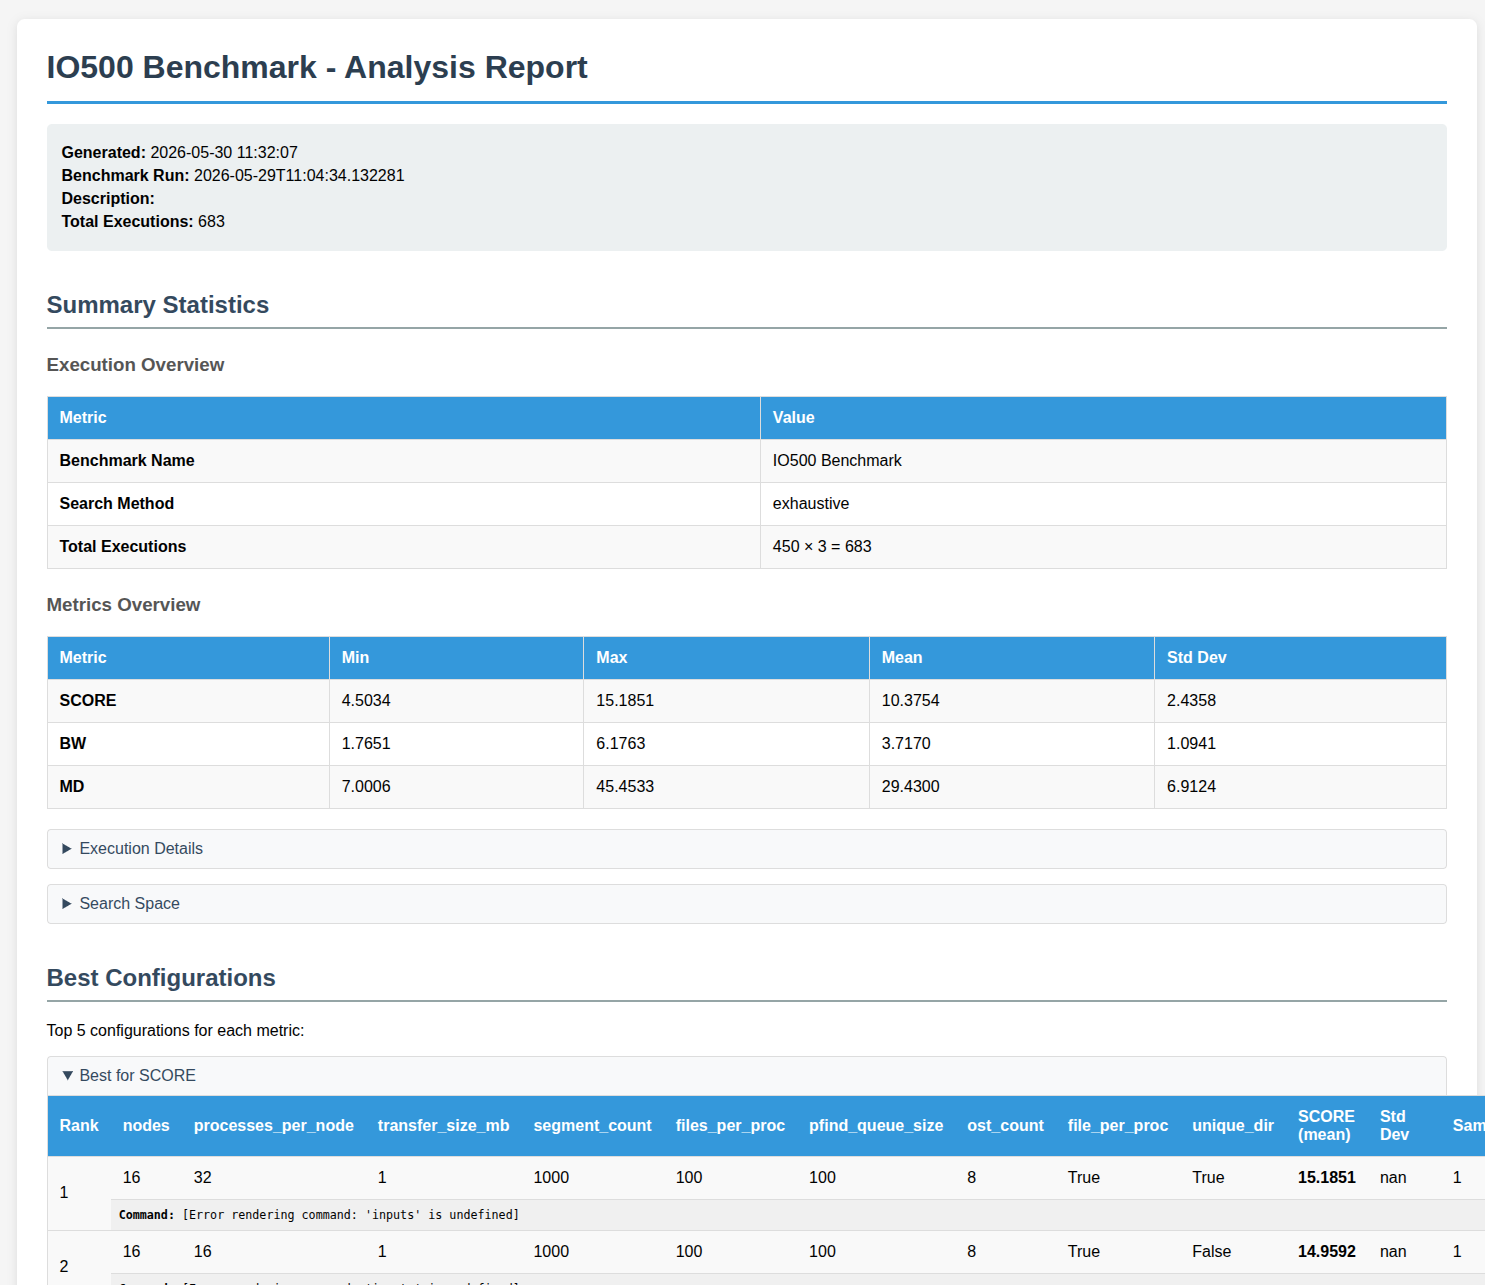
\includegraphics[height=52mm]{figures/report01.png}
    \end{column}
  \end{columns}

  \vspace{4pt}
  \begin{keybox}[width=\textwidth, top=2pt, bottom=2pt]
    \centering\footnotesize
    \faGlobe~\href{https://iops.gitlabpages.inria.fr/}{iops.gitlabpages.inria.fr}
    \;\textbar\;
    \faBox~{\ttfamily pip install iops-benchmark}
  \end{keybox}
\end{frame}

\end{document}
